In this experiment, we varied the number of source nodes, number of destination nodes and total number of nodes (partition sizes) but kept the ratio between the source nodes and the destination nodes constant. With P is size of the partition, we choose the first P/16 nodes as the source nodes, and N/2 last nodes as the destination nodes. Each node in the set of source nodes communicates with 8 nodes in the set of destination nodes. The pairing is aligned i.e. node 0 communicates with nodes (P/2, ..., P/2/7). We randomly choosing the data size for each pair of communication from 64 KB up to 8 MB of data. We experimented with 3 communication patterns: Disjoint, Overlap, Subset and 3 approaches: Optimization, Heuristic and MPI\_Alltoallv. We used only 1 MPI/PAMI rank per node. The total number of nodes P varied from 512 up to 4096 nodes. The communication throughputs are shown in Figure \ref{fig:constantr_msg}.

\begin{figure*}[!htbp]
        \centering
        \begin{subfigure}[b]{0.32\textwidth}
                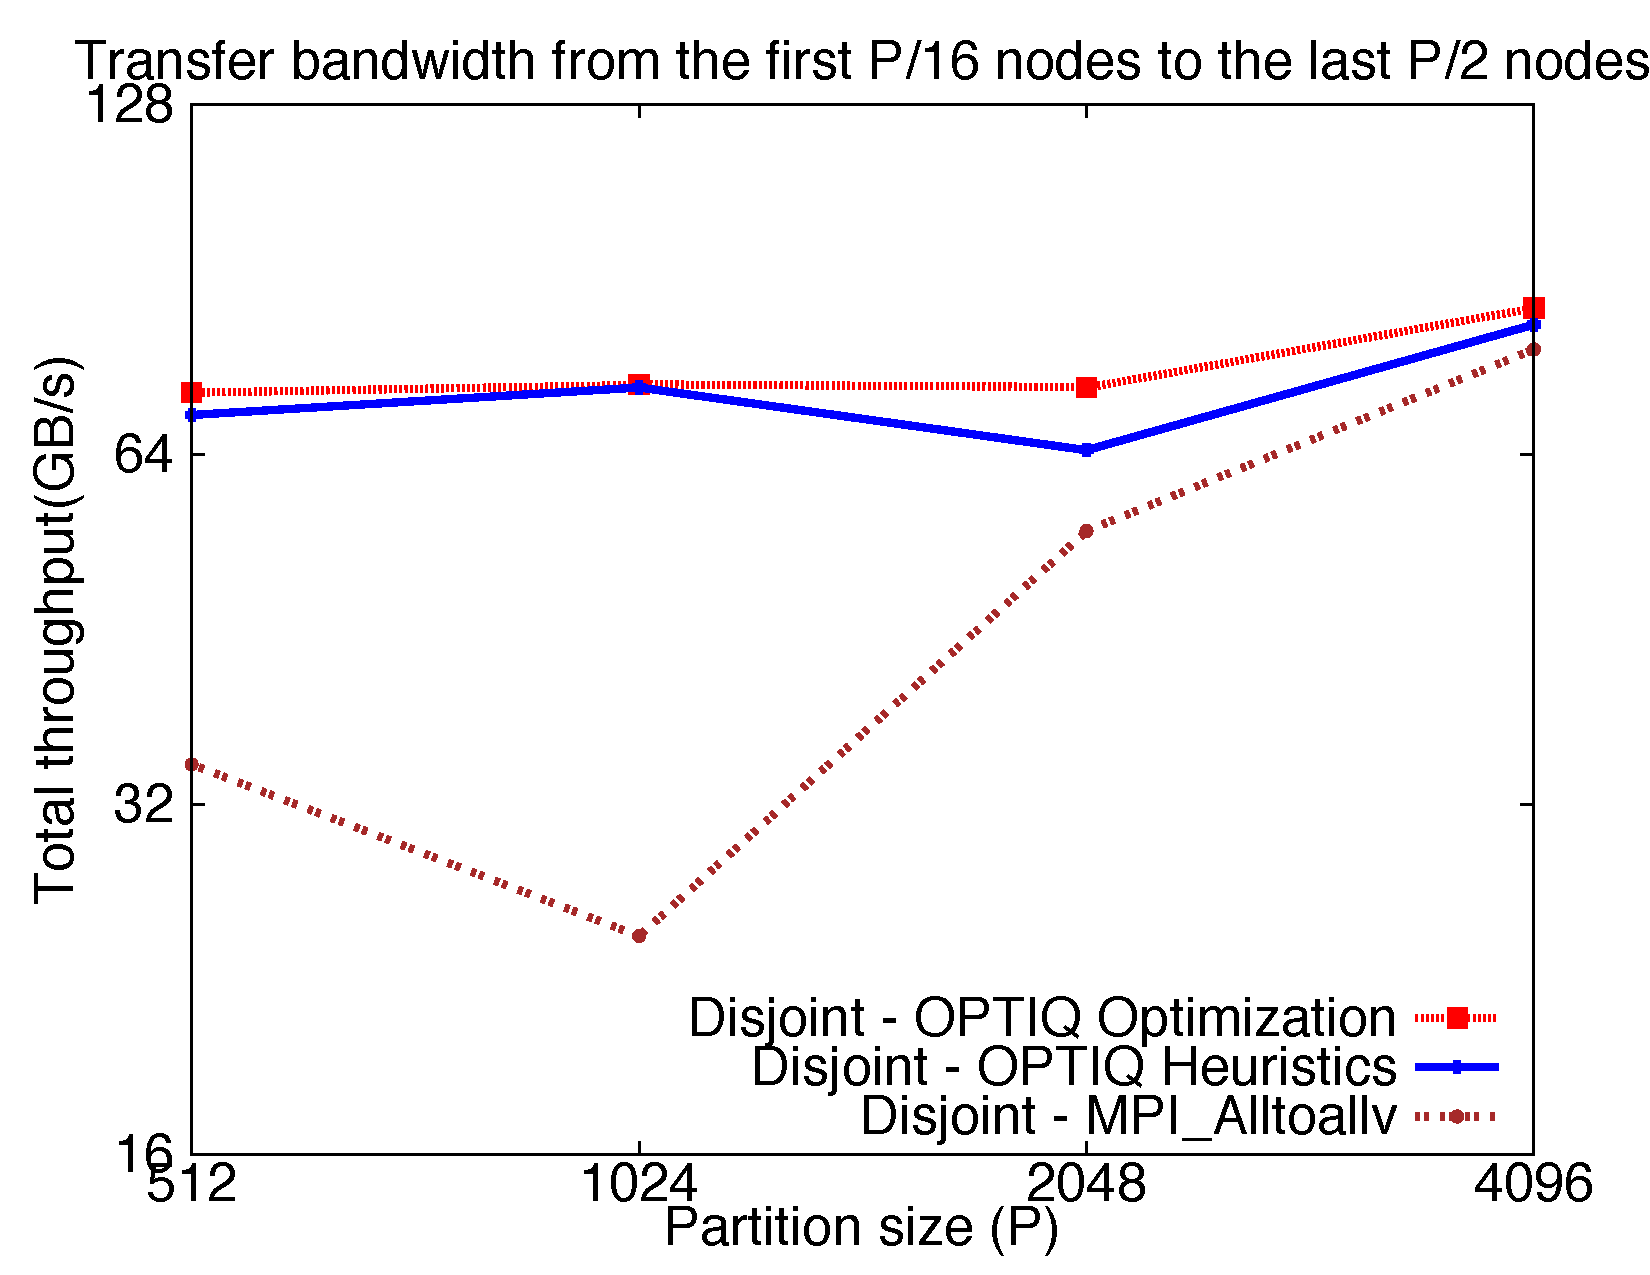
\includegraphics[width=\textwidth]{figures/constantr_disjoint_msg.pdf}
                \caption{Disjoint}
                \label{fig:constantr_disjoint_msg}
        \end{subfigure}%
        ~ %add desired spacing between images, e. g. ~, \quad, \qquad, \hfill etc.
          %(or a blank line to force the subfigure onto a new line)
        \begin{subfigure}[b]{0.32\textwidth}
                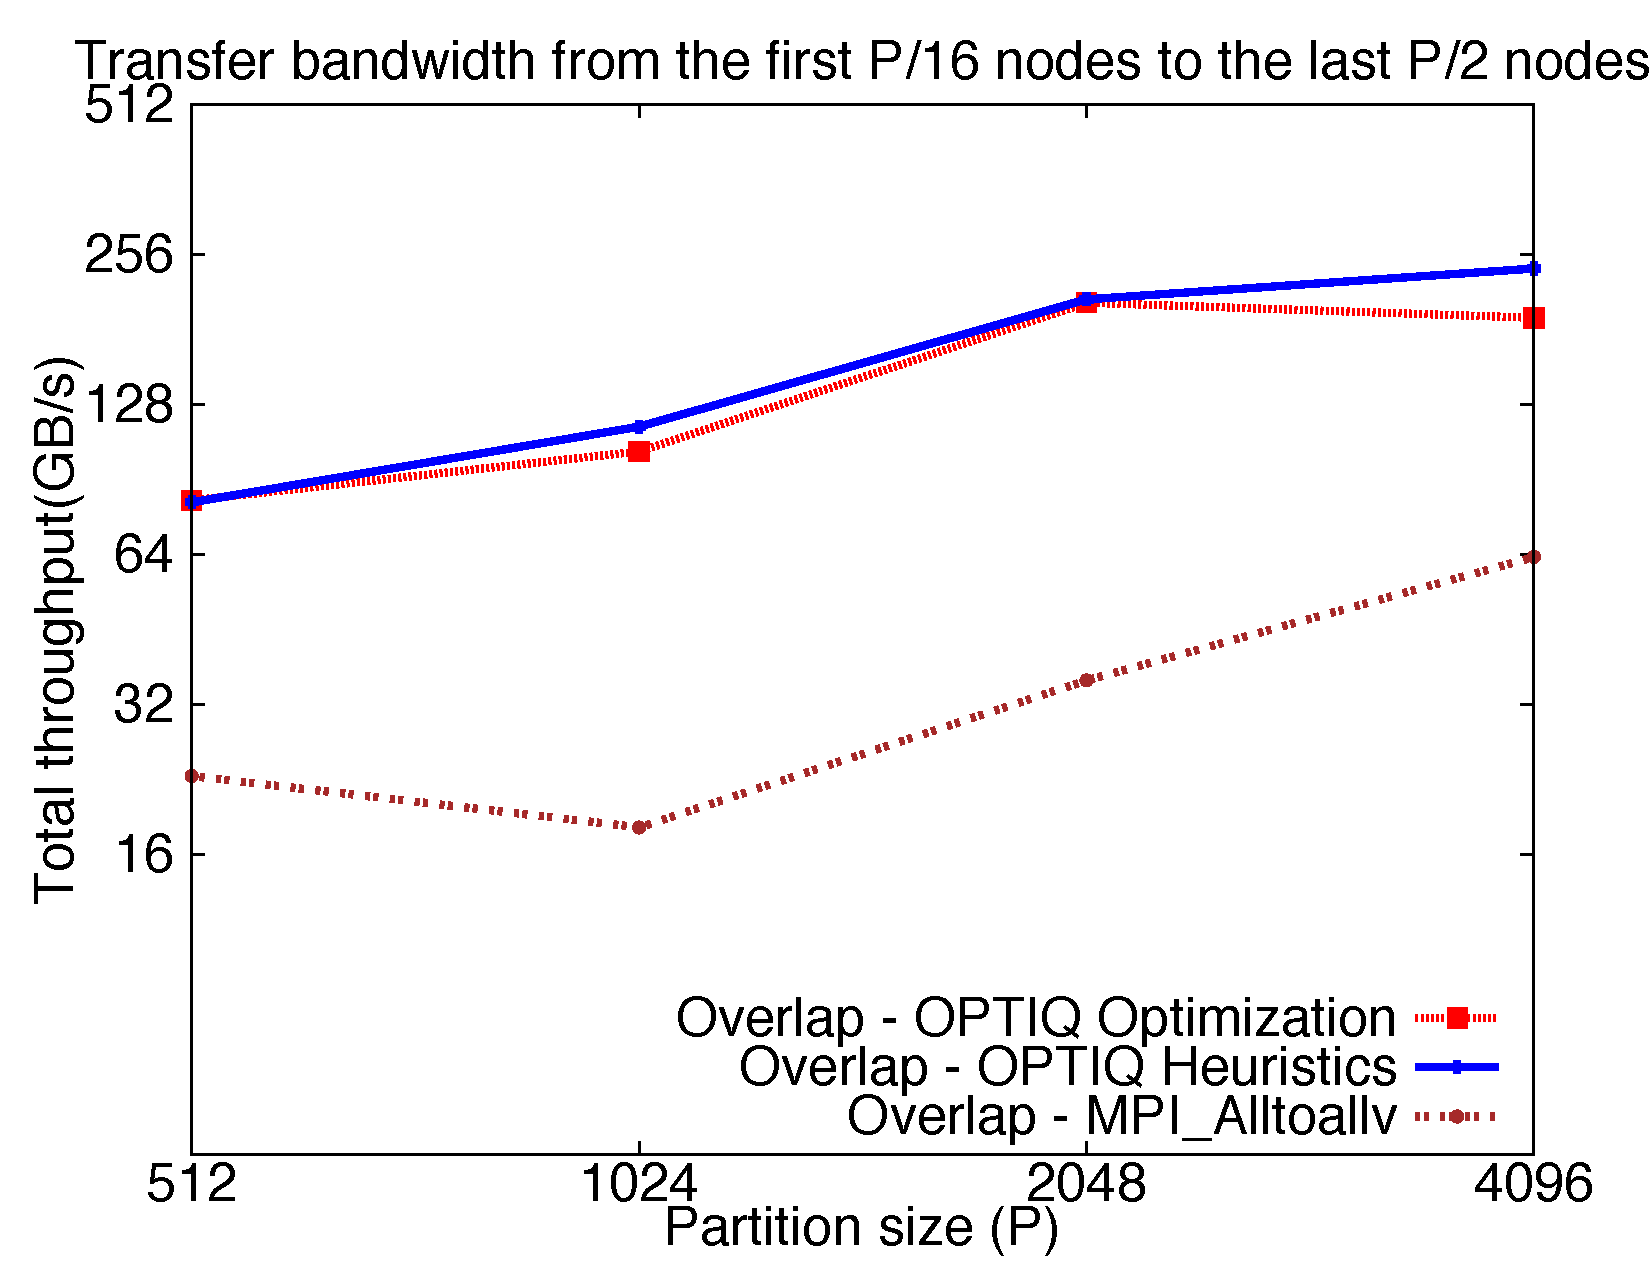
\includegraphics[width=\textwidth]{figures/constantr_overlap_msg.pdf}
                \caption{Overlap}
                \label{fig:constantr_overlap_msg}
        \end{subfigure}
        ~ %add desired spacing between images, e. g. ~, \quad, \qquad, \hfill etc.
          %(or a blank line to force the subfigure onto a new line)
        \begin{subfigure}[b]{0.32\textwidth}
                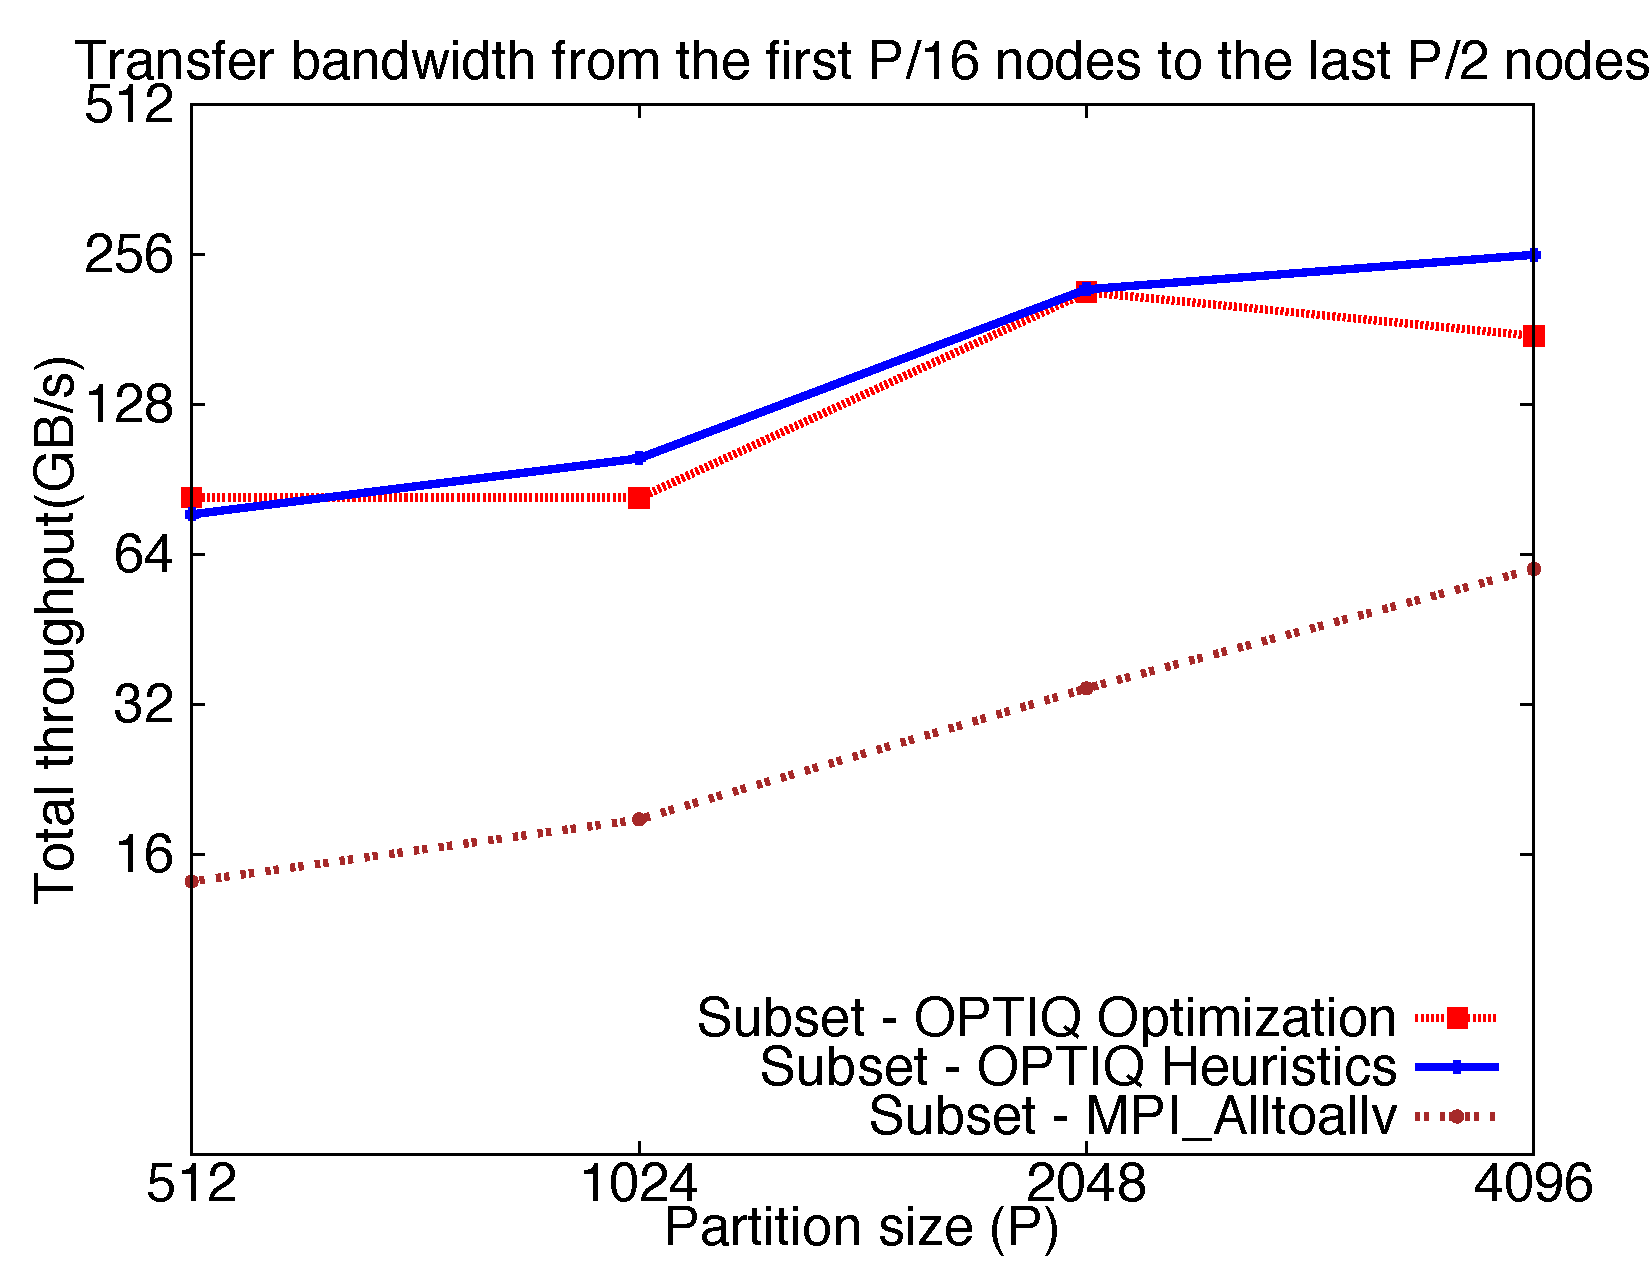
\includegraphics[width=\textwidth]{figures/constantr_subset_msg.pdf}
                \caption{Subset}
                \label{fig:constantr_subset_msg}
        \end{subfigure}
	\vspace{-0.1in}
        \caption{Varying the number of sources and destinations and total number of nodes with constant ratio}
        \label{fig:constantr_msg}
\end{figure*}

As shown in the Figure \ref{fig:constantr_msg}, in all the three communication patterns, Optimization approach and Heuristic approach have similar performance and is both significant higher than MPI\_Alltoallv in most of the experiments. In Disjoint pattern, the performance gap is close at 4096 nodes with at the other 2 patterns, the gap is quite constant showing the scalability of our approaches.

In the demonstrated experiments, both Heuristic approach and Optimization approach outperform MPI\_Alltoallv. However, this comes with a tradeoff of additional time for paths computation. In our experiments, the Heuristic approach can take from less than one second up to several seconds to compute paths. The Optimization approach can take from several second up to several hours. Thus, if communication patterns are repeated and the paths computation time can be armortized, we can use the Heuristic approach online, while the Optimization approach is suitable with off-line paths computation with patterns known prior runtime.

In the next section, we demonstrate the efficacy of our approaches through an experiment with communication patterns and data from a real application Community Earth System Model (CESM).
